\section{Introduction}\label{sec:intro}
The transfer function of an electric circuit holds important information about the circuit's response to excitation by different frequencies.
A transfer function has the form of:
\begin{equation}\label{eq:tf}
	H \left( s \right) = K { s - z \over s - p }
\end{equation}
where the values of $K$, $p$ and $z$ are determined the the circuit configuration.
The values of $s = z$ and $s = p$ are the \textit{poles} and \textit{zeros} of the transfer function and correspond to frequencies that will alter the frequency response of the circuit.

This experiment examines the frequency response of the circuit shown in Fig. \ref{fig:schematic}

\begin{figure}[tbph]
\centering
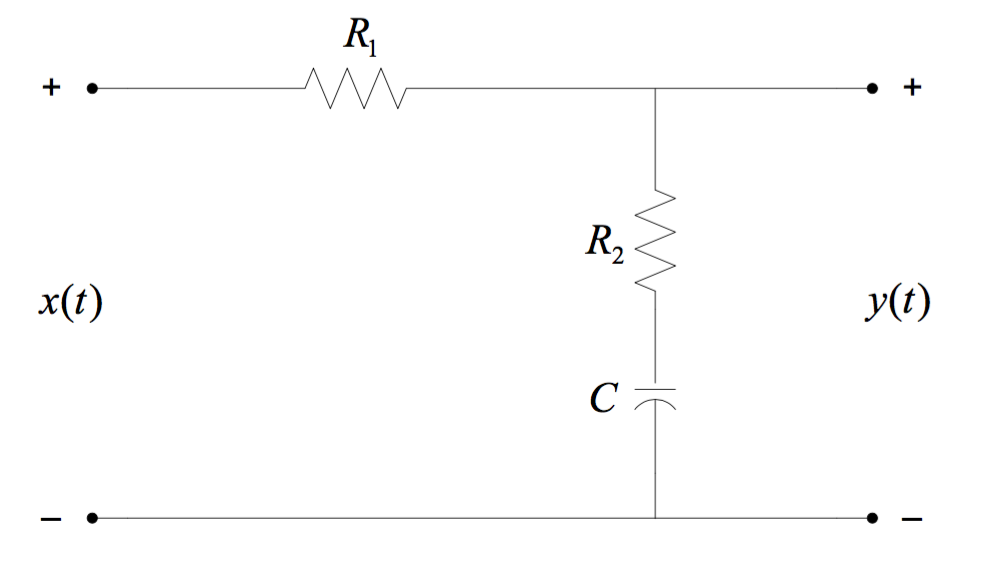
\includegraphics[width=0.7\linewidth]{graphics/lag-schematic}
\caption{Schematic of a phase lag circuit}
\label{fig:schematic}
\end{figure}

The transfer function of this circuit is:
\begin{equation}\label{eq:tf-phaselag}
H \left( s \right) = { R_2 + \frac{1}{sC} \over R_1 + R_2 + \frac{1}{sC}} = {R_2 \over R_1 + R_2 } { s + \frac{1}{C R_2} \over s + \frac{1}{C \left( R_1 + R_2 \right)} }.
\end{equation}
Comparing \eqref{eq:tf} with \eqref{eq:tf-phaselag} gives:

\begin{align}
K &= {R_2 \over R_1 + R_2 } \nonumber \\
\left|z\right| &= \frac{1}{C R_2} \label{eq:zero}\\
\left|p\right| &= \frac{1}{C \left( R_1 + R_2 \right)}. \label{eq:pole}
\end{align}

The lab manual specified that the circuit would be designed such that there was a pole at $f = \SI{1000}{\hertz}$  and a zero at $f = \SI{10000}{\hertz}$.
Using these values and the constraint $C = \SI{0.01}{\nano\farad}$, \eqref{eq:zero} and \eqref{eq:pole} yield $R_1 = \SI{1.591}{\kilo\ohm}$ and $R_2 = \SI{14.324}{\kilo\ohm}$.
$R_1$ can be realized with a standard \SI{1.6}{\kilo\ohm} resistor and $R_2$ can be realized from a \SI{10}{\kilo\ohm} resistor in series with a \SI{10}{\kilo\ohm} potentiometer tuned to \SI{4324}{\ohm}.
